\documentclass[12pt, a4paper]{article}
\usepackage[utf8]{inputenc}
\usepackage[russian]{babel}
\usepackage[pdftex]{graphicx, color}
\usepackage{amsmath}
\usepackage{amsfonts}
\usepackage{amssymb}
\usepackage{amsthm}
\usepackage[left=2cm,right=1.5cm,top=1.5cm,bottom=2cm]{geometry}
\usepackage{indentfirst}
\usepackage{hyperref}

\usepackage{setspace}
\onehalfspacing
\graphicspath{{pic/}}

\begin{document}

	\thispagestyle{empty}

	\begin{singlespace}
	\begin{titlepage}
		\begin{center}
			
\includegraphics[height = 3cm]{msu.png}

			{\scshape Московский государственный университет имени М.~В.~Ломоносова}\\
			Факультет вычислительной математики и кибернетики\\
			\centerline{\hfill\hrulefill\hrulefill\hrulefill\hrulefill\hfill}

			\vfill

			{\LARGE Отчет к четвертому заданию практикума на ЭВМ: \\  {\bfМетоды восстановления плотности распределений в задаче вычитания фона}}

			\vspace{1cm}

		\end{center}

		\vfill
		\begin{flushright}
			\textit{Студент 3 курса ВМК (317 группа):}\\
				Оспанов А.М.

			\vspace{5mm}

		\end{flushright}

		\vfill

		\begin{center}
		Москва, 2014
		\end{center}
	\end{titlepage}
	\end{singlespace}

	\tableofcontents


	\newpage
	\section{Введение}
		Данный отчет написан к четвертому заданию практикума на ЭВМ 317 группы. Тема задания:  Методы восстановления плотности распределений в задаче
вычитания фона. Отчет написан студентом 317 группы -- Оспановым Аятом.

		В данной работе были реализованы следующие методы вычитания фона: одномерная гауссиана, оценка гауссианы на лету, оценка гауссиана в 3D, EM-алгоритм восстановления парматеров смеси гауссиан. Они были применены на выборках ``Пешеходы'' и ``Траффик''. Были сделаны выводы по нахождению оптимальных параметров для каждого метода и для наглядности визуализированы.

	\newpage
	\section{Основная часть}
		\subsection{Одномерная гауссиана}
			На первом графике (при $k * \sigma = 0$) видно, что ошибок первого рода очень много (порядка 70000 пикселей из 86400), но нет ошибок 2-го рода. Т.е. при этом пороге, мы не сможем правильно определить движущиеся объекты, т.к. метод опрделеяет много шума
			\begin{center}
				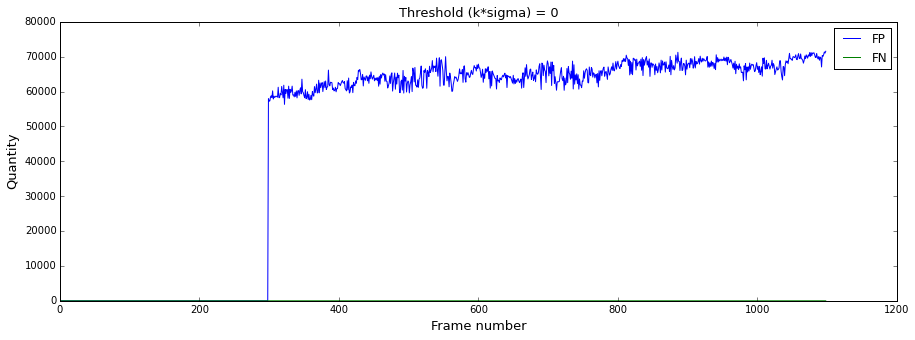
\includegraphics[width=17cm]{1par_k_0.png}
			\end{center}

			Далее (при $k * \sigma = 5, 10, 15$) ошибки первого рода снижаются, а ошибки второго рода практический не меняются и близки к нулю.
			\begin{center}
				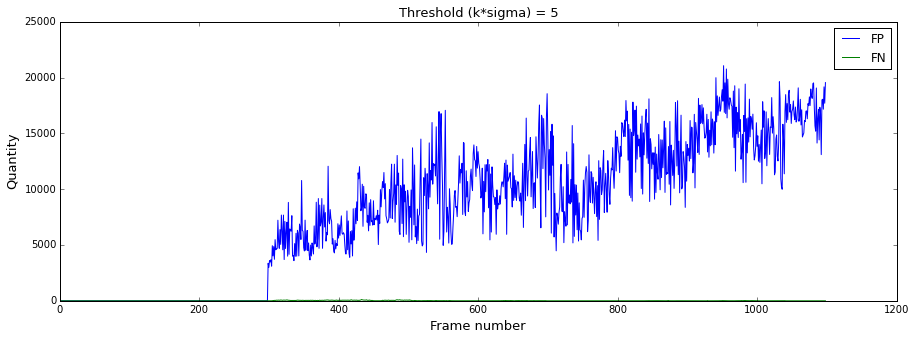
\includegraphics[width=17cm]{1par_k_5.png}
			\end{center}
			\begin{center}
				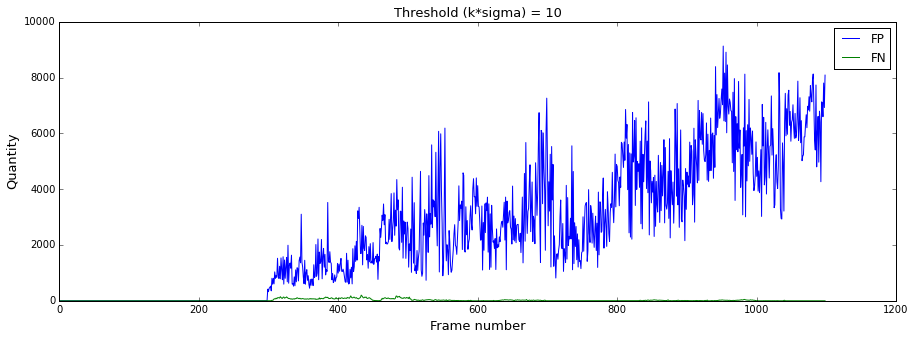
\includegraphics[width=17cm]{1par_k_10.png}
			\end{center}
			\begin{center}
				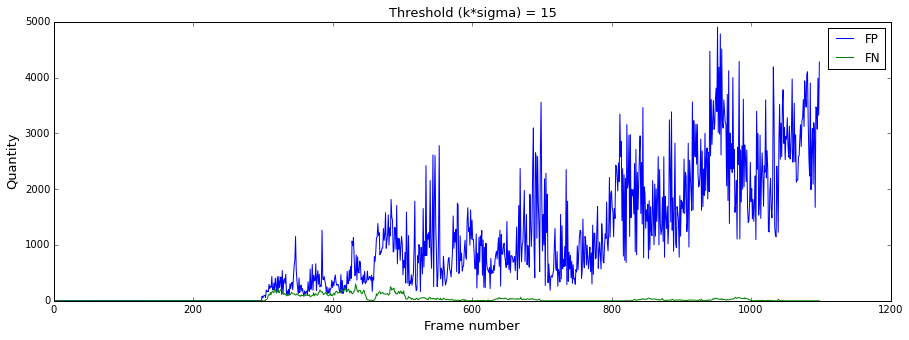
\includegraphics[width=17cm]{1par_k_15.png}
			\end{center}

			Начиная с порога равного 20, ошибки второго рода резко начинают расти, а ошибки первого рода снижаются.
			\begin{center}
				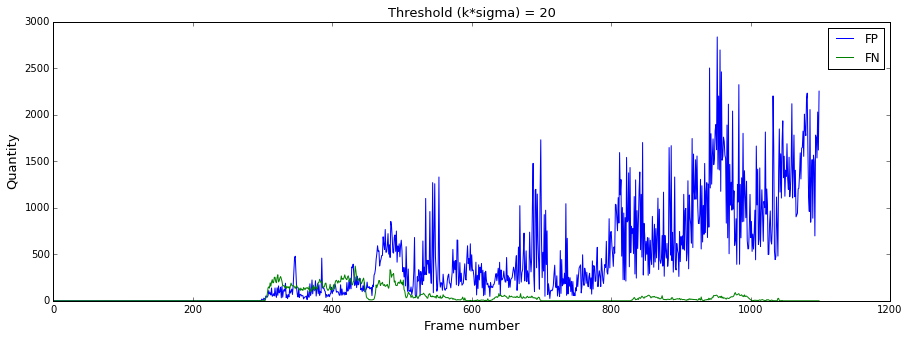
\includegraphics[width=17cm]{1par_k_20.png}
			\end{center}
			\begin{center}
				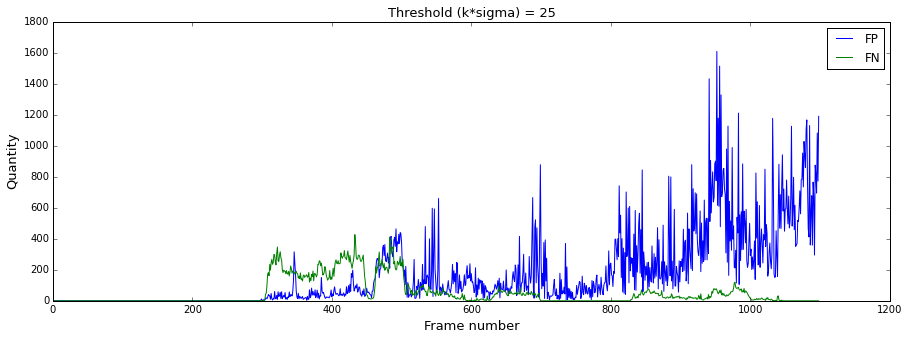
\includegraphics[width=17cm]{1par_k_25.png}
			\end{center}

			Начиная с порога раного 30, ошибок второго рода начинает становиться больше, чем первого рода. Но при классификации лучше всего сказать, что объект движется, нежели, чем объект не движется. Т.е. нам важно, чтобы ошибок второго рода, было меньше первого. Но при этом нужно найти оптимум, такой, что, и ошибки первого рода, и второго рода были как можно меньше. Из всех графиков видно, что такой оптимум достигается при пороге равной 30-35.
			\begin{center}
				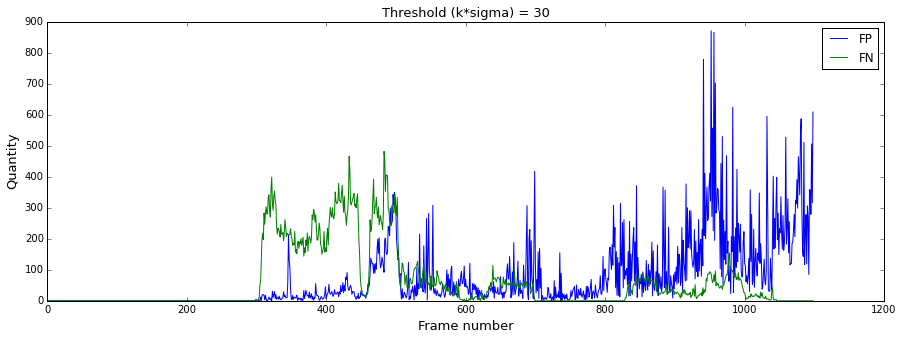
\includegraphics[width=17cm]{1par_k_30.png}
			\end{center}
			\begin{center}
				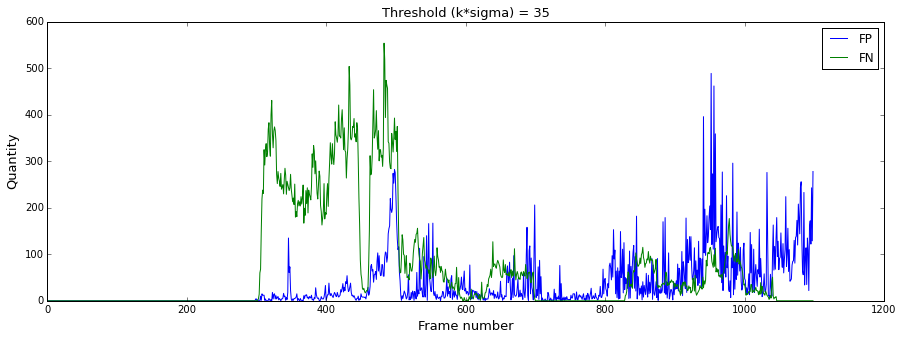
\includegraphics[width=17cm]{1par_k_35.png}
			\end{center}
			\begin{center}
				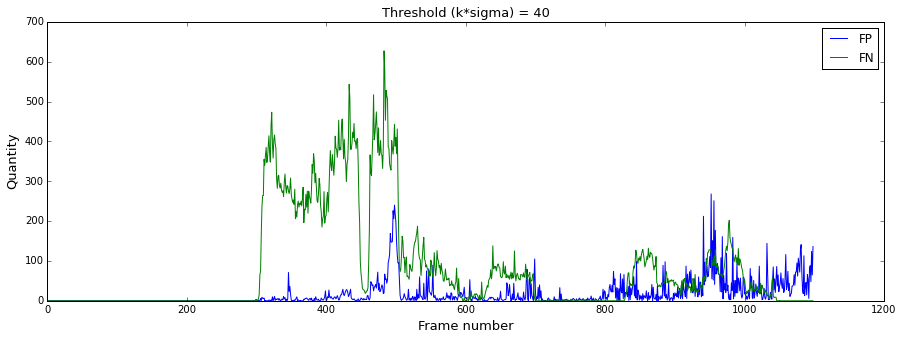
\includegraphics[width=17cm]{1par_k_40.png}
			\end{center}
			\begin{center}
				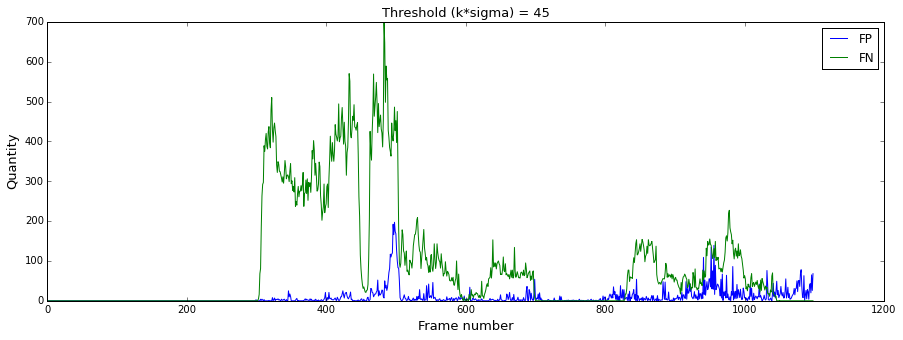
\includegraphics[width=17cm]{1par_k_45.png}
			\end{center}

			Далее на картинках представлены кадры из видео, где можно увидеть результат данного метода при $k * \sigma = 30$
			\begin{center}
				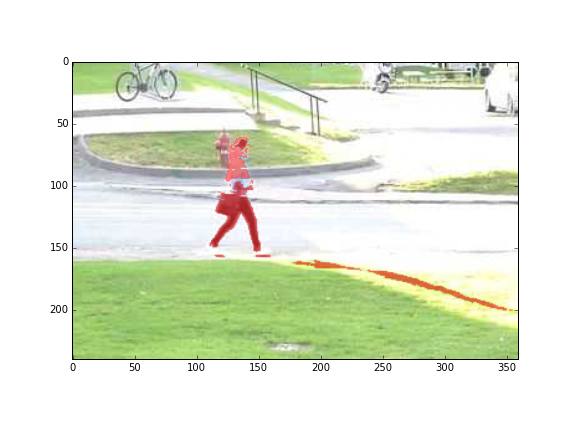
\includegraphics[width=8.5cm]{1par_vid_0.png}
				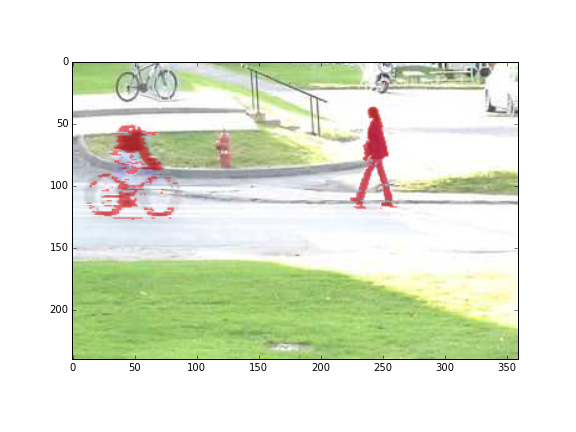
\includegraphics[width=8.5cm]{1par_vid_1.png}
			\end{center}

			Те области движущихся объектов, цвета которых близки к фоновому цвету в соответствующих областях, определяются как фон. А если цвета различимы, то объект определятся хорошо. В целом данный метод хорошо работает и быстро.

			Далее можно увидеть качество данного метода
			\begin{center}
				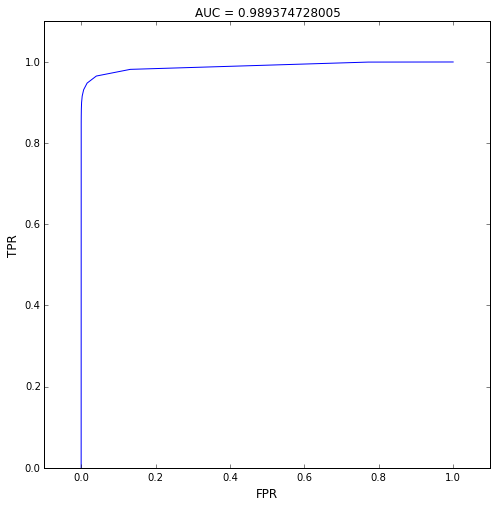
\includegraphics[width=8.5cm]{1par_auc.png}
			\end{center}

		\newpage
		\subsection{Оценка гауссианы на лету}
			Из первого графика (при $k = 0$) можно сделать те же выводы, что и для первого графика (при $k * \sigma = 0$) предыдущего метода
			\begin{center}
				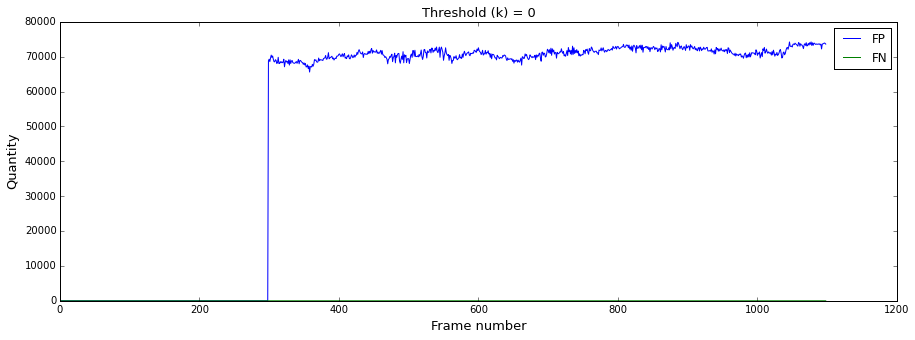
\includegraphics[width=17cm]{2par_k_0.png}
			\end{center}

			Далее (при $k = 5$) ошибки первого рода естественно снижаются, а ошибки второго рода практический близки к нулю.
			\begin{center}
				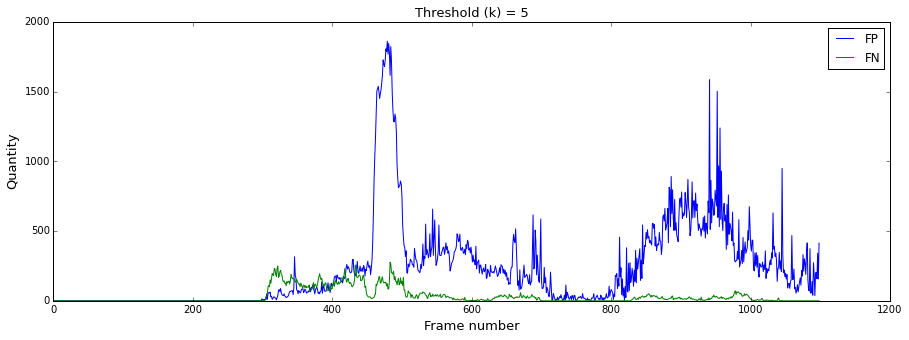
\includegraphics[width=17cm]{2par_k_5.png}
			\end{center}

			Начиная с $k = 10$ ошибки второго рода резко увеличиваются, а ошибки первого рода стремятся к нулю.
			\begin{center}
				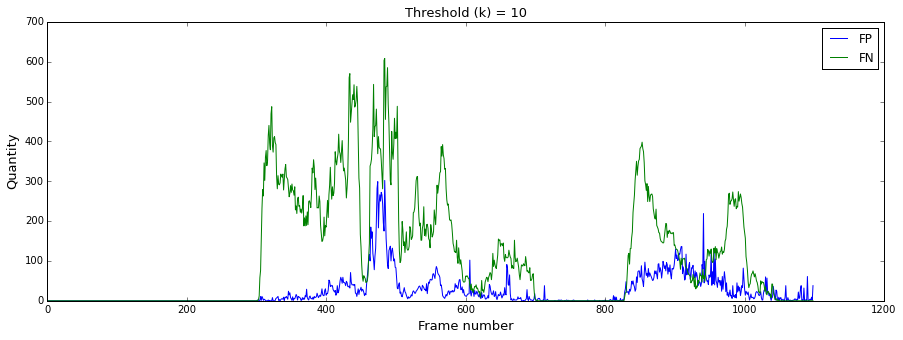
\includegraphics[width=17cm]{2par_k_10.png}
			\end{center}
			\begin{center}
				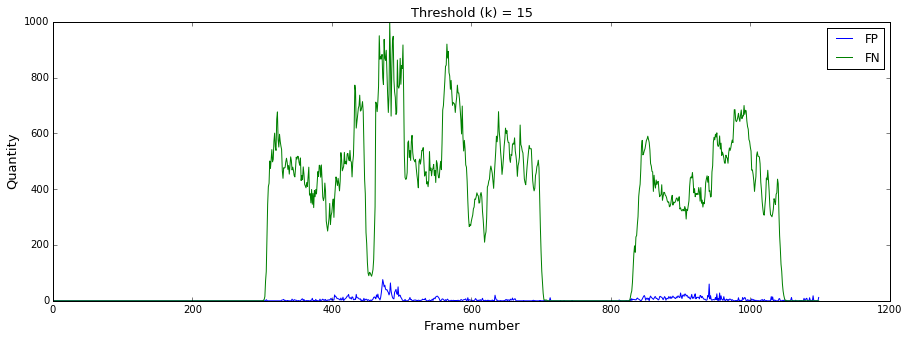
\includegraphics[width=17cm]{2par_k_15.png}
			\end{center}

			Начиная с порога равного 20, ошибки второго рода становятся постоянными, а ошибки первого рода нулевыми (тоже постоянными).
			\begin{center}
				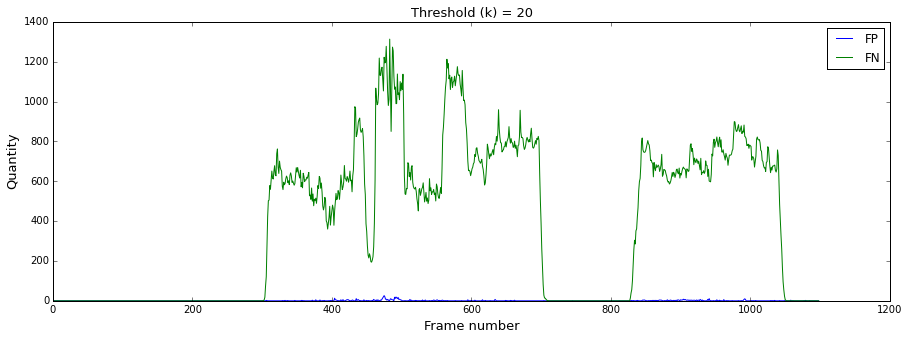
\includegraphics[width=17cm]{2par_k_20.png}
			\end{center}
			\begin{center}
				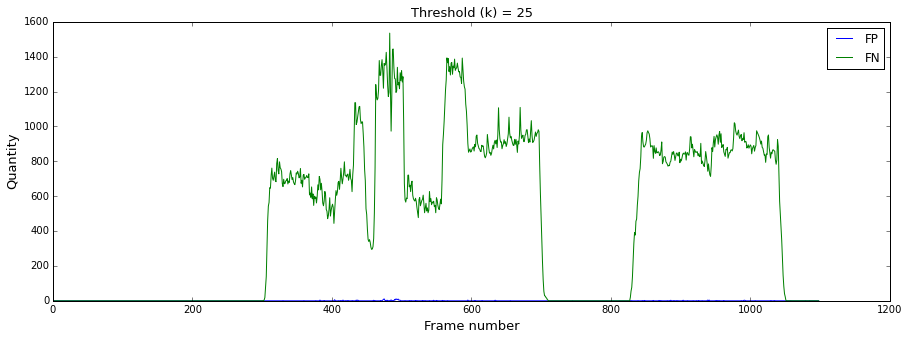
\includegraphics[width=17cm]{2par_k_25.png}
			\end{center}

			Результаты при $k = [10, 25]$ показывают, что мы упустили интервал в котором расположен ``хороший'' порог. При $k = 5$ и $k = 10$ мы видели хороший результат, следовательно надо искать в этом интервале:
			\begin{center}
				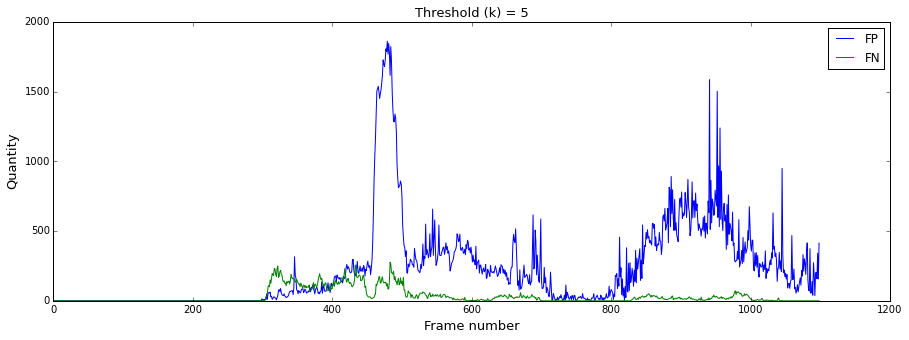
\includegraphics[width=17cm]{2par_k_5.png}
			\end{center}
			\begin{center}
				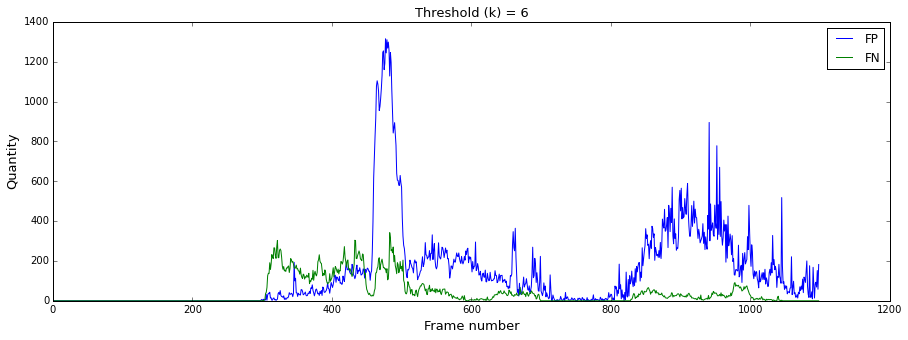
\includegraphics[width=17cm]{2par_k_6.png}
			\end{center}
			\begin{center}
				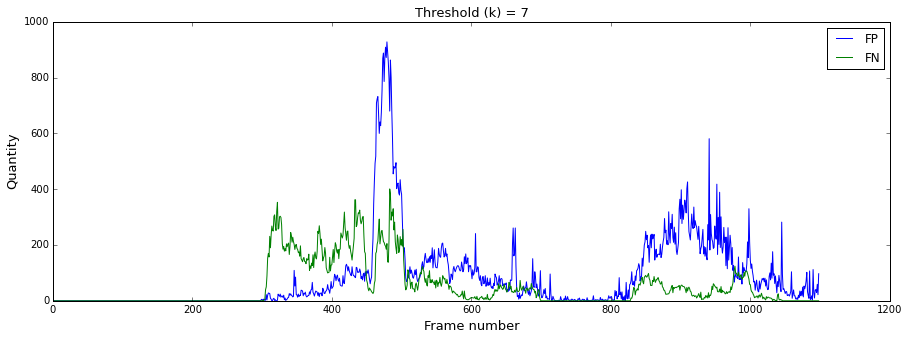
\includegraphics[width=17cm]{2par_k_7.png}
			\end{center}
			\begin{center}
				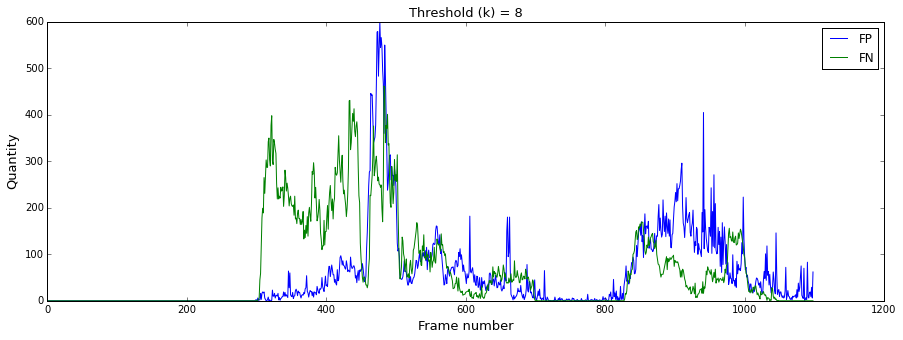
\includegraphics[width=17cm]{2par_k_8.png}
			\end{center}
			\begin{center}
				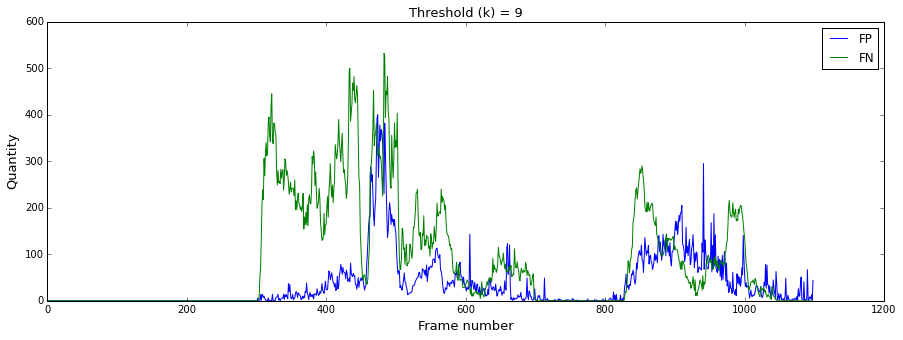
\includegraphics[width=17cm]{2par_k_9.png}
			\end{center}

			Из предыдущих графиков видно, что оптимум достигается при $k ~ 8$

			Далее на картинках представлены кадры из видео, где можно увидеть результат данного метода при $k = 8.5$
			\begin{center}
				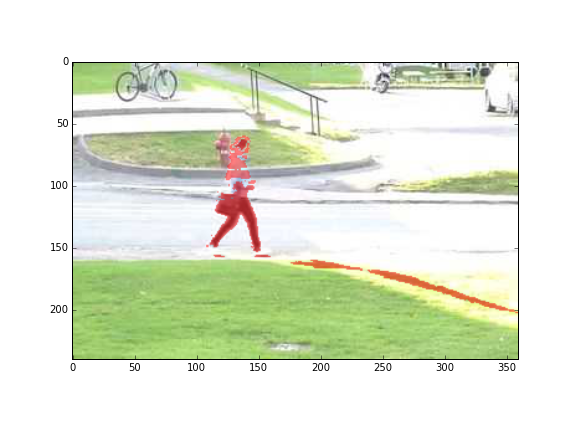
\includegraphics[width=8.5cm]{2par_vid_0.png}
				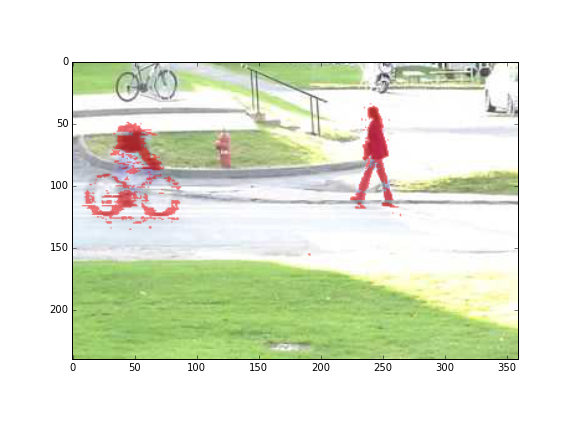
\includegraphics[width=8.5cm]{2par_vid_1.png}
			\end{center}

			Результаты такие же, как и в первом методе

			Далее можно увидеть качество данного метода
			\begin{center}
				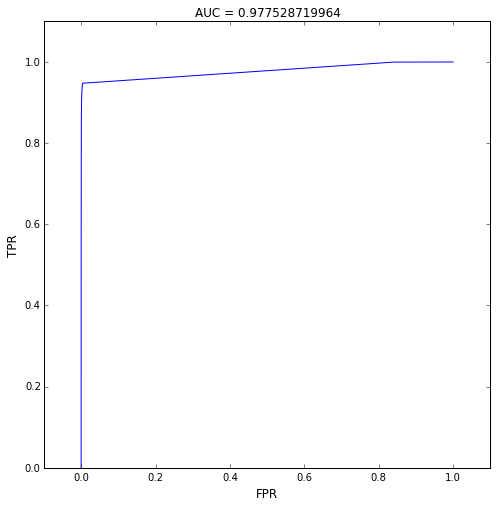
\includegraphics[width=8.5cm]{2par_auc.png}
			\end{center}

		\newpage
		\subsection{Теперь в 3D!}
			{\bf RGB вариант}

			Далее приведены графики зависимости ошибок первого и второго рода данного метода в зависимости от номера кадра. По ним можно увидеть, что с ростом порога увеличивается ошибка первого рода, но уменьшается ошибка второго рода. Начиная со значения порога равного 0.1 метод работает очень плохо. Из всех представленных прогов надо выбрать оптимальный. Из графиков можно увидеть, что оптимальный параметр находится между $k = 1e-100$ и $k = 1e-50$
			\begin{center}
				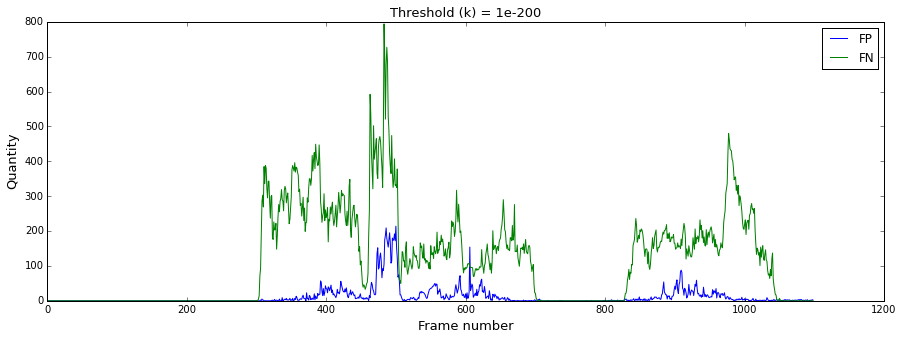
\includegraphics[width=17cm]{3_par_rgb_k_1e_200.png}
			\end{center}
			\begin{center}
				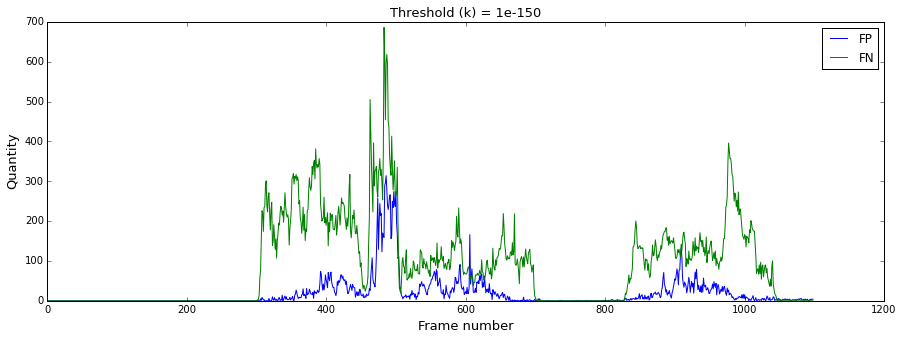
\includegraphics[width=17cm]{3_par_rgb_k_1e_150.png}
			\end{center}
			\begin{center}
				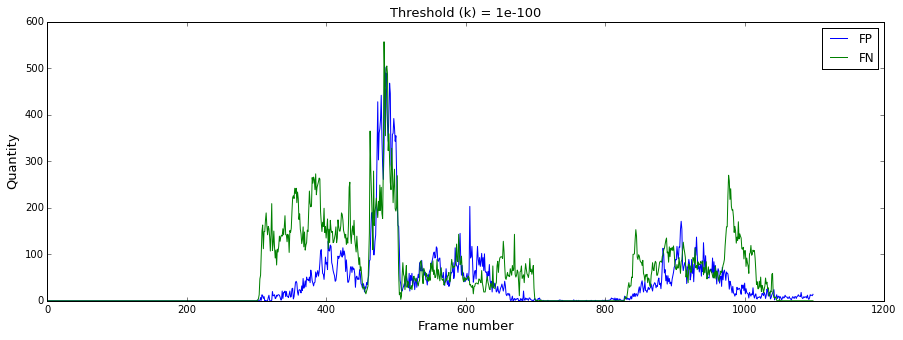
\includegraphics[width=17cm]{3_par_rgb_k_1e_100.png}
			\end{center}
			\begin{center}
				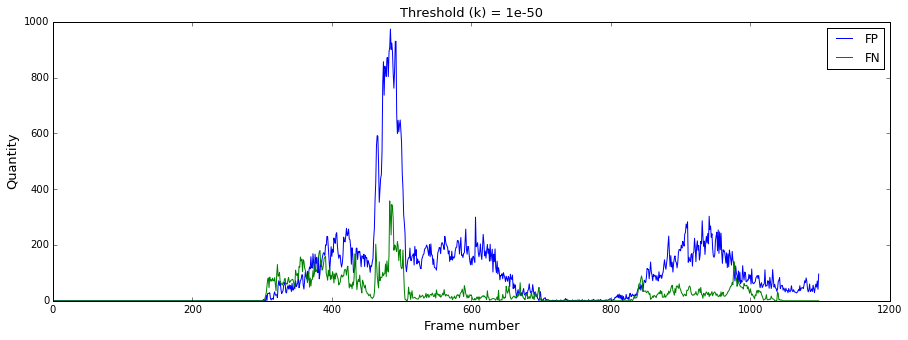
\includegraphics[width=17cm]{3_par_rgb_k_1e_50.png}
			\end{center}
			\begin{center}
				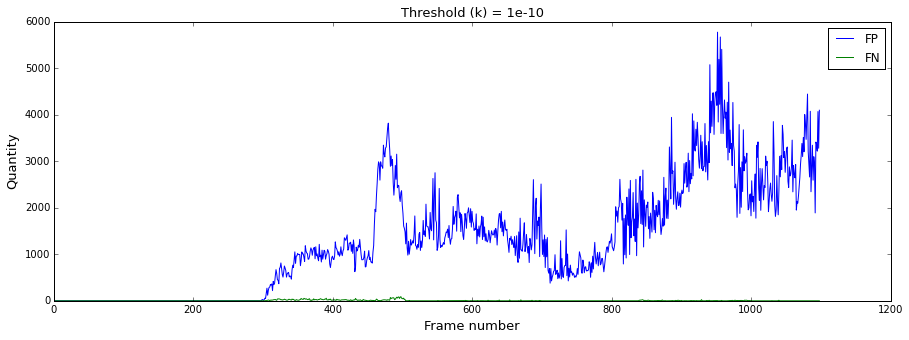
\includegraphics[width=17cm]{3_par_rgb_k_1e_10.png}
			\end{center}
			\begin{center}
				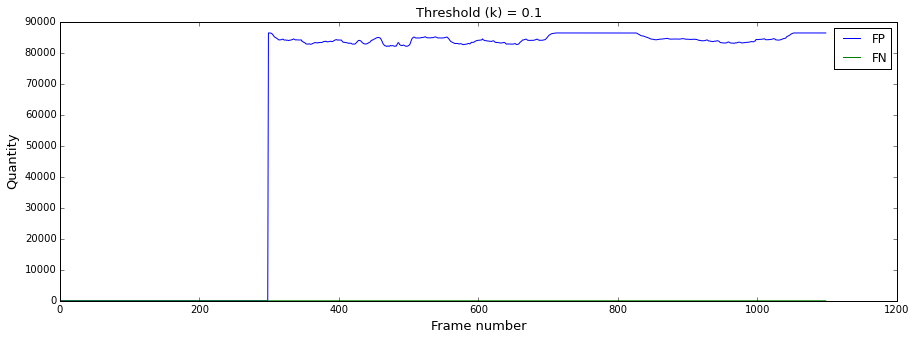
\includegraphics[width=17cm]{3_par_rgb_k_1e_1.png}
			\end{center}
			\newpage
			Из графиков мы выяснили, что оптимальный порог находится в отрезке \\ $k = [1e-100, 1e-50]$. Давайте посмотрим кадры для $k = 1e-70$:

			\begin{center}
				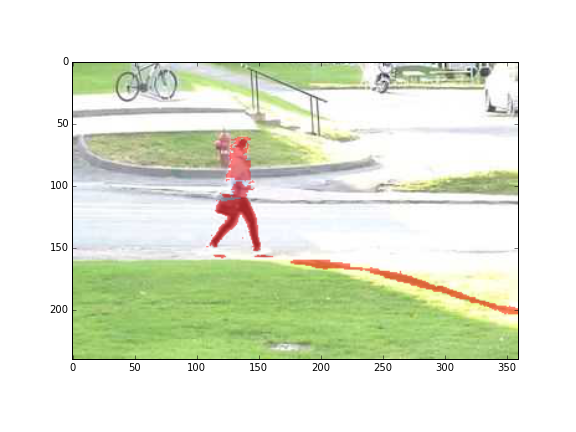
\includegraphics[width=8.5cm]{3_par_rgb_vid_0.png}
				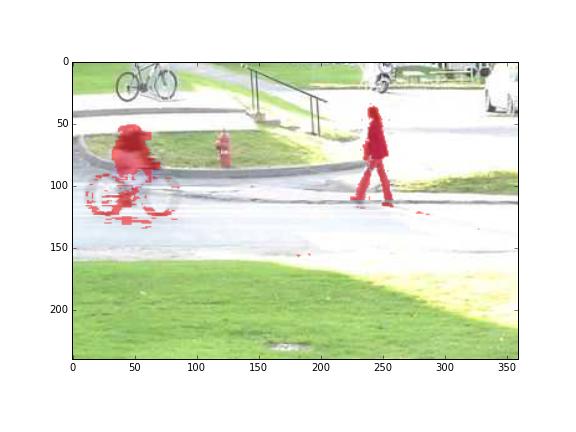
\includegraphics[width=8.5cm]{3_par_rgb_vid_1.png}
			\end{center}

			Результаты улучшились, по сравнению с предыдущими методами. Это хорошо!

			Далее можно увидеть график ROC-кривую для данного метода
			\begin{center}
				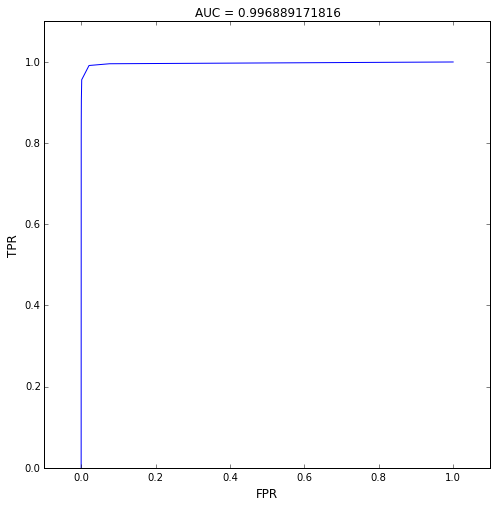
\includegraphics[width=8.5cm]{3_par_rgb_auc.png}
			\end{center}


			\newpage
			{\bf\centering HSV вариант}

			После конвертации из RGB в HSV графики особо не поменялись. Изменился лишь порог, при котором этот график похож на соответственный график для RGB.
			\begin{center}
				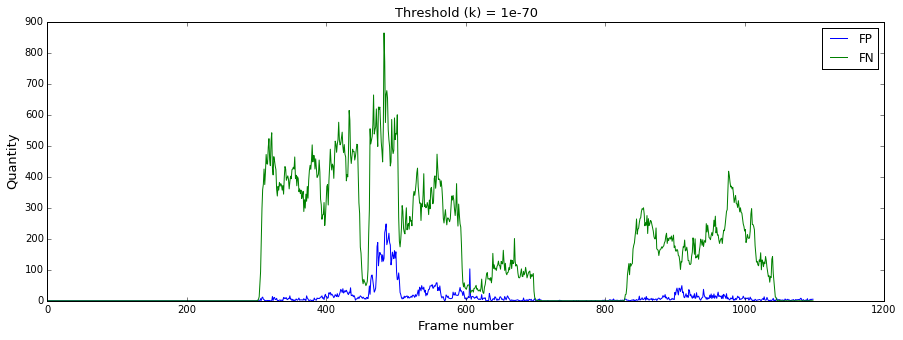
\includegraphics[width=17cm]{3_par_hsv_k_1e-70.png}
			\end{center}
			\begin{center}
				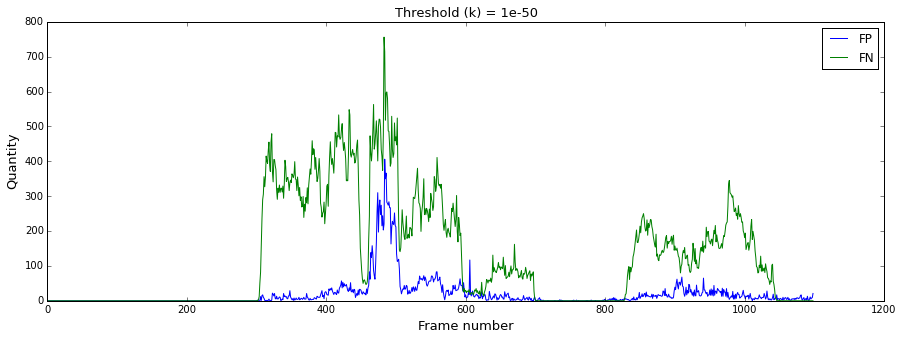
\includegraphics[width=17cm]{3_par_hsv_k_1e-50.png}
			\end{center}
			\begin{center}
				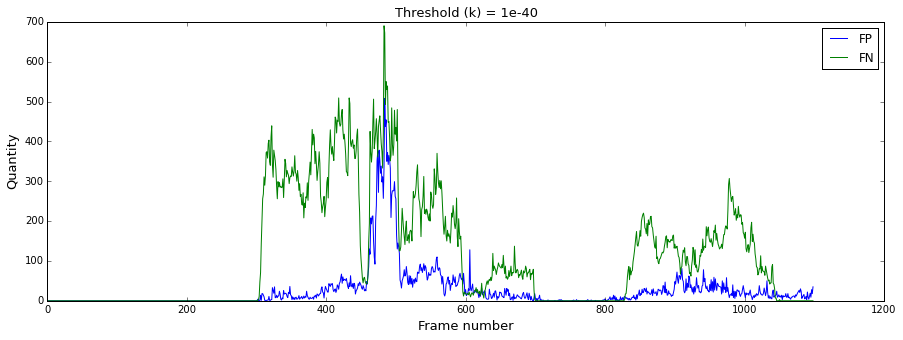
\includegraphics[width=17cm]{3_par_hsv_k_1e-40.png}
			\end{center}
			\begin{center}
				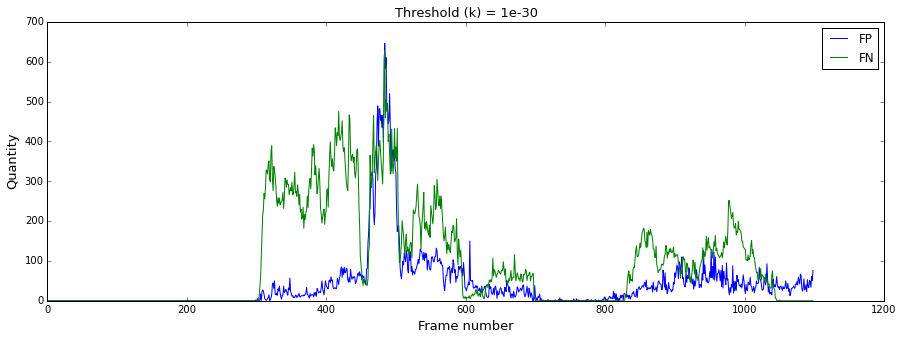
\includegraphics[width=17cm]{3_par_hsv_k_1e-30.png}
			\end{center}
			\begin{center}
				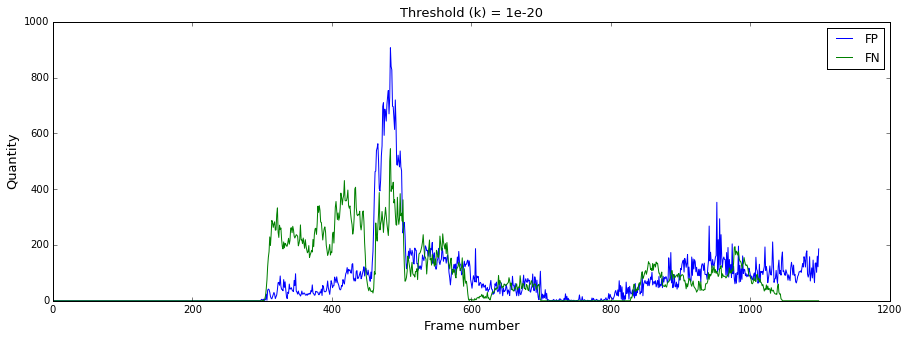
\includegraphics[width=17cm]{3_par_hsv_k_1e-20.png}
			\end{center}
			\begin{center}
				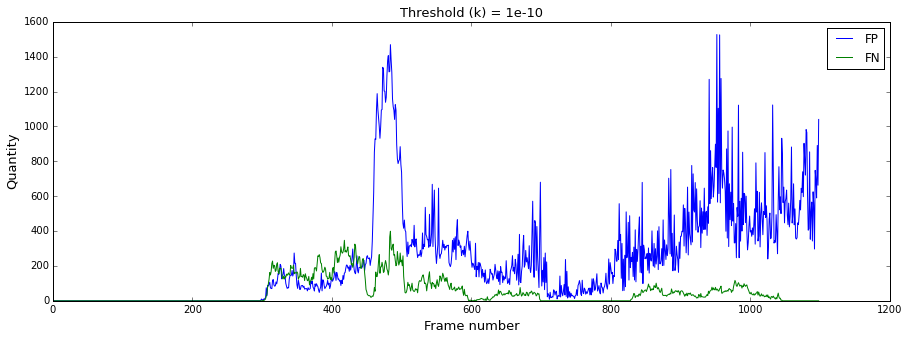
\includegraphics[width=17cm]{3_par_hsv_k_1e-10.png}
			\end{center}
			\begin{center}
				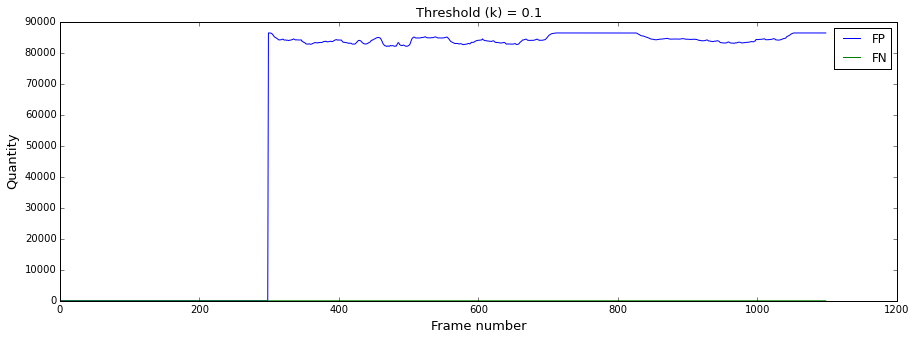
\includegraphics[width=17cm]{3_par_hsv_k_0_1.png}
			\end{center}

			Хоть графики и похожи, но качество изменилось. Из следующих кадров можно увидеть, что есть части движущихся объектов, отнесенных к фону, но которые определялись при RGB. Т.е. для данных входных данных, HSV ухудшает точность.
			
			RGB
			\begin{center}	
				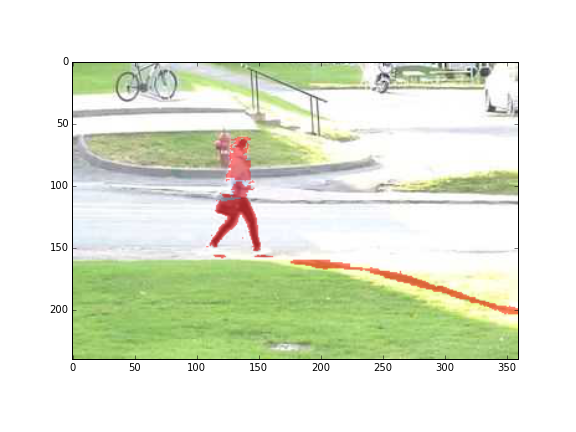
\includegraphics[width=8.5cm]{3_par_rgb_vid_0.png}
				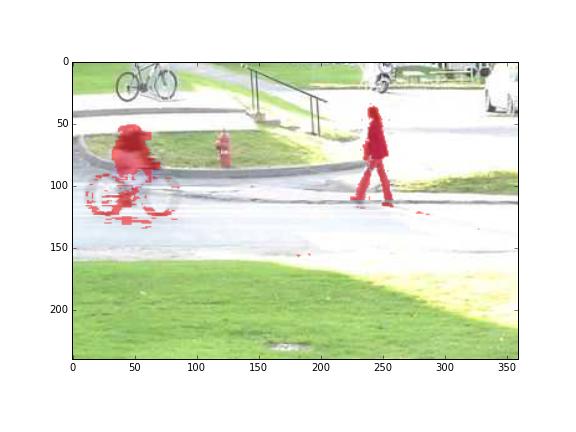
\includegraphics[width=8.5cm]{3_par_rgb_vid_1.png}
			\end{center}

			HSV
			\begin{center}
				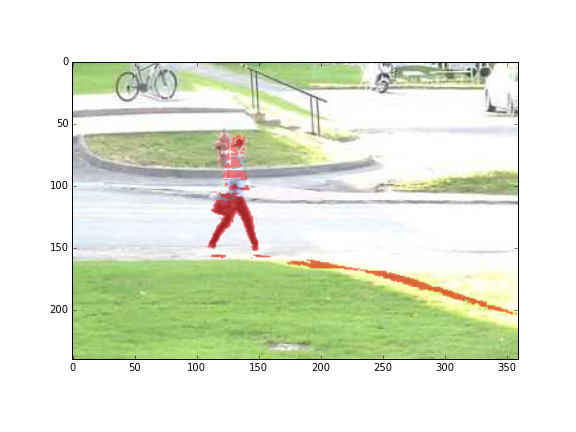
\includegraphics[width=8.5cm]{3_par_hsv_vid_0.png}
				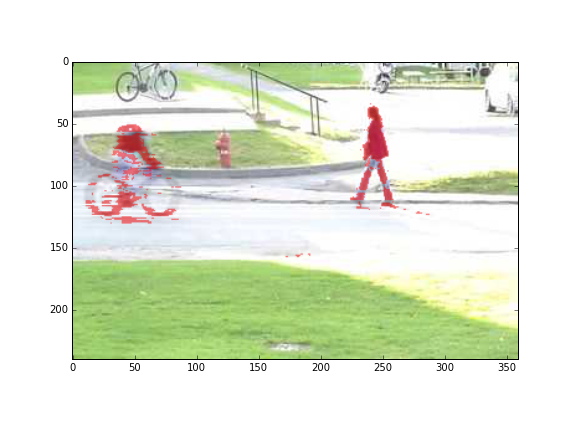
\includegraphics[width=8.5cm]{3_par_hsv_vid_1.png}
			\end{center}

			Ухудшение можно увидеть и на ROC-кривой (для RGB AUC $\approx$ 0.9969):
			\begin{center}
				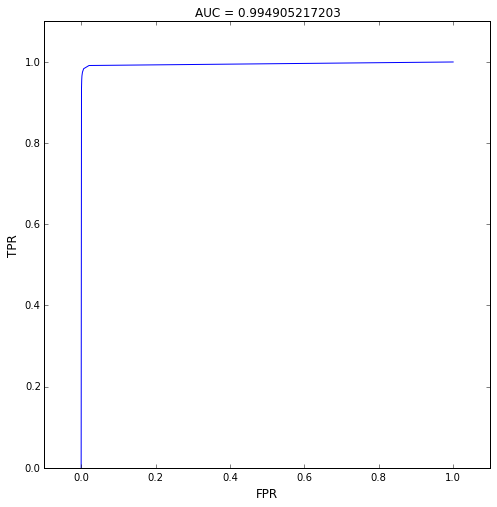
\includegraphics[width=8.5cm]{3_par_hsv_auc.png}
			\end{center}

		\newpage
		\subsection{Смесь гауссиан}
			{\bf Исследование EM алгоритма}

			В следующей таблице изображена хорошо разделимая выборка и результат работы алгортима K-средних. На этой выборке мы будет исследовать работу EM алгоритма.
			% Хорошо разделимая выборка

			\begin{center}
			\begin{tabular}{ c  c }
				Выборка & К-средних \\

				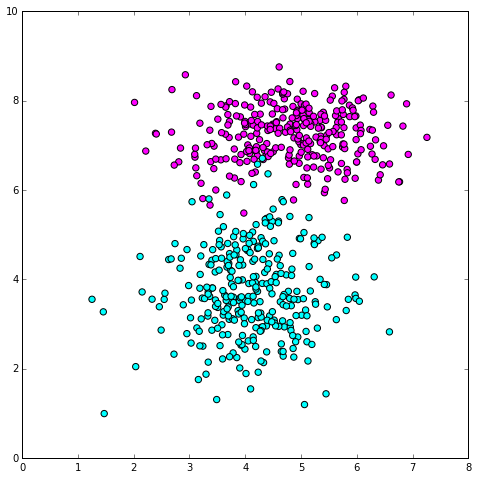
\includegraphics[width=5cm]{4par_orig.png} &
				\includegraphics[width=5cm]{4par_kmean.png} \\
			\end{tabular}
			\end{center}

			Давайте исследуем на этой выборке работу EM алгоритма в зависимости от начальных данных.

			\begin{center}
			\begin{tabular}{ c c c }
				\hline
				К-средних & Случайные & Слуайные из выборки \\

				15 итераций & 37 итераций & 14 итераций \\

				\hline

				\includegraphics[width=5cm]{4par_kminit_em.png} &
				\includegraphics[width=5cm]{4par_rdinit_EM.png} &
				\includegraphics[width=5cm]{4par_rdinitx_EM.png} \\

				\includegraphics[width=5cm]{4par_kminit_MLE.png} &
				\includegraphics[width=5cm]{4par_rdinit_MLE.png} &
				\includegraphics[width=5cm]{4par_rdinitx_MLE.png} \\

				\hline
			\end{tabular}
			\end{center}

			Из таблицы видно, что независимо от начальных данных, метод сработал хорошо и одинаково. Но количество итераций, хоть и не на много, но отличается. За меньшее число итераций сработали методы инициализированные данными полученные методом K-редних и случайными данными выбранными из выборки.

			\newpage
			А в следующей таблице изображена плохо разделимая выборка и результат работы алгортима K-средних на ней. На этой выборке мы будет исследовать работу EM алгоритма.
			% Плохо разделимая выборка

			\begin{center}
			\begin{tabular}{c c}
				Выборка & К-средних \\

				\includegraphics[width=5cm]{4par_orig_bad.png} &
				\includegraphics[width=5cm]{4par_kmean_bad.png} \\
			\end{tabular}
			\end{center}

			Давайте исследуем на этой выборке работу EM алгоритма в зависимости от начальных данных.

			\begin{center}
			\begin{tabular}{c c c}
				\hline
				К-средних & Случайные & Слуайные из выборки \\

				773 итераций & 770 итераций & 460 итераций \\

				\hline

				\includegraphics[width=5cm]{4par_kminit_em_bad.png} &
				\includegraphics[width=5cm]{4par_rdinit_EM_bad.png} &
				\includegraphics[width=5cm]{4par_rdinitx_EM_bad.png} \\

				\includegraphics[width=5cm]{4par_kminit_MLE_bad.png} &
				\includegraphics[width=5cm]{4par_rdinit_MLE_bad.png} &
				\includegraphics[width=5cm]{4par_rdinitx_MLE_bad.png} \\

				\hline
			\end{tabular}
			\end{center}

			Из таблицы видно, что лучше всех сработал метод инициализированный случайными данными из выборки (т.к. выборка состояла из одинаковых количеств элементов в каждом распределении). И к тому же в данном случае метод сработал за 460 итераций против 770. А в остальных случаях картинки более менее похожи и количество итераций тоже совпадают с некоторой погрешностью. 

			Из результатов по двум выборкам можно сделать вывод о том, что если выбирать случайные элементы из выборки как начальное приближение, то EM-алгоритм работает быстро и более точно.

	\newpage
	\section{Заключение}
		В этой задаче, мы исследовали методы вычитания фона по отдельности. В случае статической камеры мы исслеовали три метода. Сравним их. Для этого взглянем на ROC-кривые.
		\begin{center}
			\begin{tabular}{c c}
				\hline
				Одномерная гауссиана & Оценка гауссианы на лету \\


				\includegraphics[width=8cm]{1par_auc.png} &
				\includegraphics[width=8cm]{2par_auc.png} \\
				
				\hline
				3D гауссиана (RGB) & 3D гауссиана (HSV) \\
				\includegraphics[width=8cm]{3_par_rgb_auc.png} &
				\includegraphics[width=8cm]{3_par_hsv_auc.png} \\

				\hline
			\end{tabular}
		\end{center}

		Из таблицы видно, что по точности лучше всех работает метод ``3D гауссиана'' при пространстве цветов RGB, но данный метод работает достаточно долго (порядка 10 мин), следующим по точности идет метод ``Одномерная гауссиана''. Но время работы данного метода не превосходит 1 минуты. Т.е. более оптимальным по критерию точность-время будет метод ``Одномерная гауссиана''.

		К сожалению запустить алгоритм EM на выборке с динамической камерой не удалось (работает очень долго), и после работы получаются шумы (не удалось отладить). Следовательно не удалось сделать выводы на счет данного метода.

		\begin{center}
			\includegraphics[width=15cm]{4par_vid.png}
		\end{center}
		
\end{document}
